% ----------------------------------------------------------
% Teste test4_1_e25b64class10_20231212_004403
% ----------------------------------------------------------
\subsubsection{Teste test4_1_e25b64class10_20231212_004403 - AlexNet (Is That a Santa)}

Informações utilizadas para o treinamento.

\begin{table}[ht]
   \centering
   \caption{Treinamento}
   \label{tab:modelos}
   \begin{tabular}{| c | c | }
      \hline 
      \textbf{Informação} & \textbf{Descrição} \\
      \hline \hline 
      Rede & AlexNet \\
      \hline
      Número de épocas & 25\\
      \hline
      Tamanho do lote & 64\\
      \hline
      Taxa inicial & 0.012 \\
      \hline
      Taxa de decaimento & 0.0006 \\
      \hline
      Total de classes & 10\\
      \hline
      Dataset & CIFAR-10\\
      \hline
   \end{tabular} 
\end{table}

Resultados obtidos após treinamento.

\begin{tabular}{lrrrr}
\toprule
  Unnamed: 0 &  precision &  recall &  f1-score &   support \\
\midrule
    airplane &   0.836557 &   0.865 &  0.850541 &  1000.000 \\
  automobile &   0.900000 &   0.909 &  0.904478 &  1000.000 \\
        bird &   0.751491 &   0.756 &  0.753739 &  1000.000 \\
         cat &   0.644645 &   0.644 &  0.644322 &  1000.000 \\
        deer &   0.822245 &   0.791 &  0.806320 &  1000.000 \\
         dog &   0.740704 &   0.737 &  0.738847 &  1000.000 \\
        frog &   0.861139 &   0.862 &  0.861569 &  1000.000 \\
       horse &   0.859281 &   0.861 &  0.860140 &  1000.000 \\
        ship &   0.895055 &   0.887 &  0.891010 &  1000.000 \\
       truck &   0.868000 &   0.868 &  0.868000 &  1000.000 \\
    accuracy &   0.818000 &   0.818 &  0.818000 &     0.818 \\
   macro avg &   0.817912 &   0.818 &  0.817897 & 10000.000 \\
weighted avg &   0.817912 &   0.818 &  0.817897 & 10000.000 \\
\bottomrule
\end{tabular}


\begin{figure}[ht]
 \begin{center}
   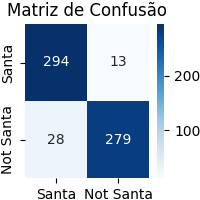
\includegraphics[scale=1]{tests/test4_1_e25b64class10_20231212_004403/confusion_matrix.png}
  \caption{Matriz de Confusão}
  \label{fig:fig03}
 \end{center}
\end{figure}

\begin{figure}[ht]
 \begin{center}
   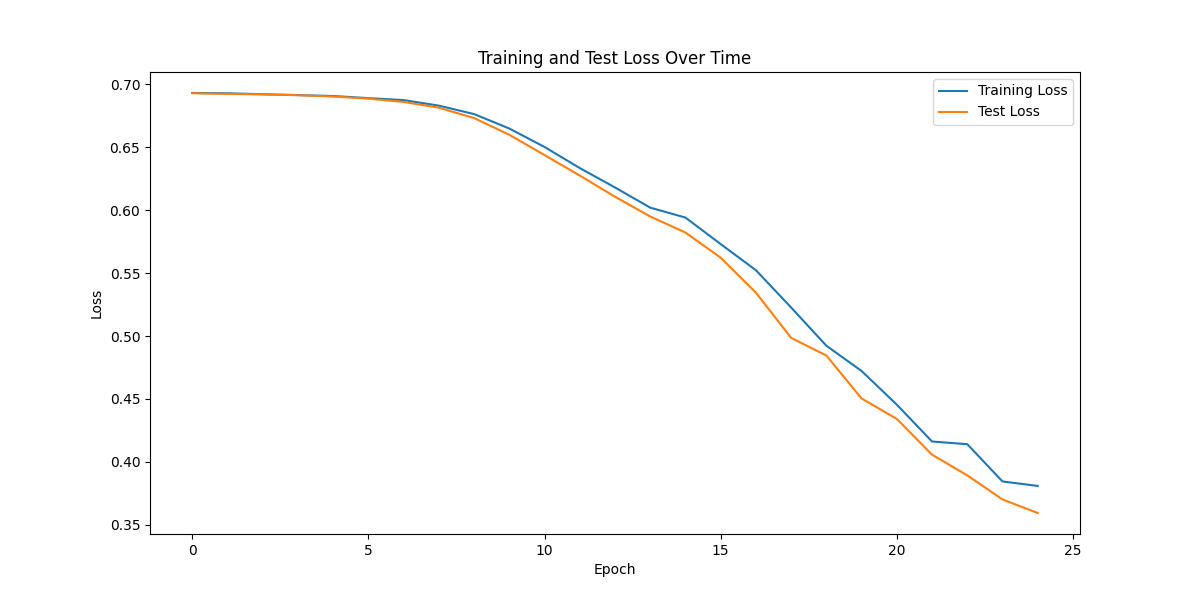
\includegraphics[scale=0.8]{tests/test4_1_e25b64class10_20231212_004403/loss_over_time.png}
  \caption{Gráfico de Perda}
  \label{fig:fig04}
 \end{center}
\end{figure}
